\beginsong{Im Silberbirkenland}[wuw={aus Kanada}, pfii={58}, pfiii={50}]

\beginverse
\endverse
\centering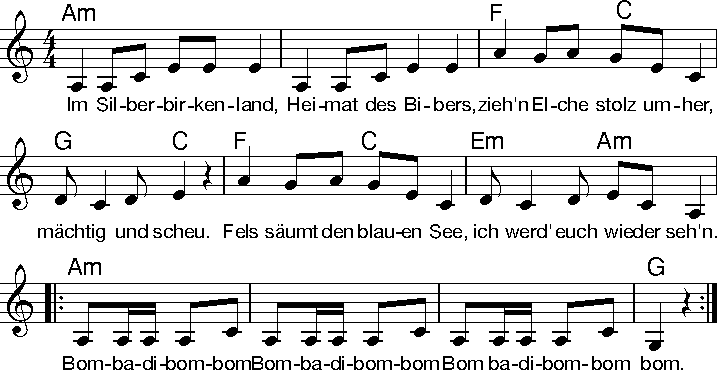
\includegraphics[width=1\textwidth]{Noten/Lied052.pdf}	

\beginverse
\[Am]Nach dir mein Herz sich sehnt fern von den Bergen;
\[F]Ich kehr' zu \[C]euch zurück, \[G]Hügel des \[C]Nordens.
\endverse

\beginchorus
\[F]Fels säumt den \[C]blauen See;
Ich \[Em]werd' euch wieder\[Am]seh'n.
\lrep \[Am]Bom badi bom bom \rrep \rep{4} \[G]
\endchorus

\beginverse
^Schnell wie ein Silberfisch gleitet mein Rindenboot
^Über den ^Strom dahin ^trägt es mich ^fort.
\endverse
\renewcommand{\everychorus}{\textnote{\bf Refrain (wdh.)}}

\beginchorus
\endchorus

\beginverse
^Hinter dem blauen See bau' ich mein Wigwam
^Dort an der ^Wasserscheid ^ruhig und ^still.
\endverse

%\beginchorus
%\endchorus

\endsong

\beginscripture{}
''Im Silberbirkenland'' stammt von dem kanadischen Indianerlied ''Land of the Silver Birch''. Die genaue Herkunft ist unklar.
\endscripture

\begin{intersong}
\ifthenelse{\boolean{pics}}{
    %\centering\includegraphics[width=1\textwidth]{Bilder/imsilberbirkenland_irena.png}
    \ThisLLCornerWallPaper{0.95}{Bilder/imsilberbirkenland_irena.png}
}{}
\end{intersong}